\documentclass{amsart}          

% PACKAGES ~~~~~~~~~~~~~~~~~~~~

\usepackage{amsfonts}
\usepackage{amssymb}  
\usepackage{amsthm} 
\usepackage{amsmath} 
\usepackage{caption}
\usepackage[inline]{enumitem}
\setlist{itemsep=0em, topsep=0em, parsep=0em}
\setlist[enumerate]{label=(\alph*)}
\usepackage{etoolbox}
\usepackage{stmaryrd} 
\usepackage{graphicx}
\usepackage[table, dvipsnames]{xcolor}

\author{Daniel Cicala}
\title{Homework Example}

\begin{document}
\maketitle{}

Throughout the semester, you will be given exercises for
which you must submit your answer as a fully written and
final-draft-quality document.  This may be typed or
handwritten. \emph{Expect to write several drafts} before
arriving at something good enough. Feedback on how to
improve drafts can be obtained in office hours.

This current document serves to provide an example of what
is expected and to provide a grading rubric. Observe that
the example solution is written in complete, grammatical
sentences with any mathematical expressions embedded into
the writing.  If you are unsure how to treat a mathematical
expression as a grammatical object, read it out loud and
follow your instinct.  Expressions like `$ 5x+3 $' are nouns
and symbols like `$ = $' or `$ \leq $' are verbs.

Additional examples of how to write mathematical content can
be found in Examples found in each chapter of the textbook.

\vfill
\noindent\rule{\textwidth}{1pt}
\vfill

\textbf{Grading rubric}

\begin{center}
  \begin{tabular}{|l|p{5cm}|p{5cm}|}
    \hline
    \rowcolor{cyan!30}
    \textbf{Score}
    & \textbf{Mathematics (25\%)}
    & \textbf{Writing (75\%)}
    \\
    \hline
    0
          & No meaningful progress towards the correct answer
                        & Incomprehensible. Scratch work.\\
    \rowcolor{cyan!15}
    1
          & Incorrect methods used. Major mistakes
                        & Minor exposition, but no grammatical structure. No
        logical flow to response. \\
    2
          & Correct methods indentified. Major mistakes.
                        & Poor exposition and grammatical structure. Poor
        logical flow. \\
    \rowcolor{cyan!15}
    3
          & Correct method and minor mistakes. Good progress to
      the correct answer.
                        & Clear exposition, few grammatical mistakes, and
        comprehensible logical flow. \\
    4
          & Correct method and no mistakes.
                        & Excellent exposition that contains to grammatical
        mistakes and clear logical flow.\\
    \hline                          
  \end{tabular}
\end{center}

\vfill
\noindent\rule{\textwidth}{1pt}
\vfill

\textbf{Example:}

Find the inverse of the function $ f(x)= 5x^3 + 7 $.

\vfill
\pagebreak

\noindent
\textbf{Here is a well-written solution:}
\begin{center}
  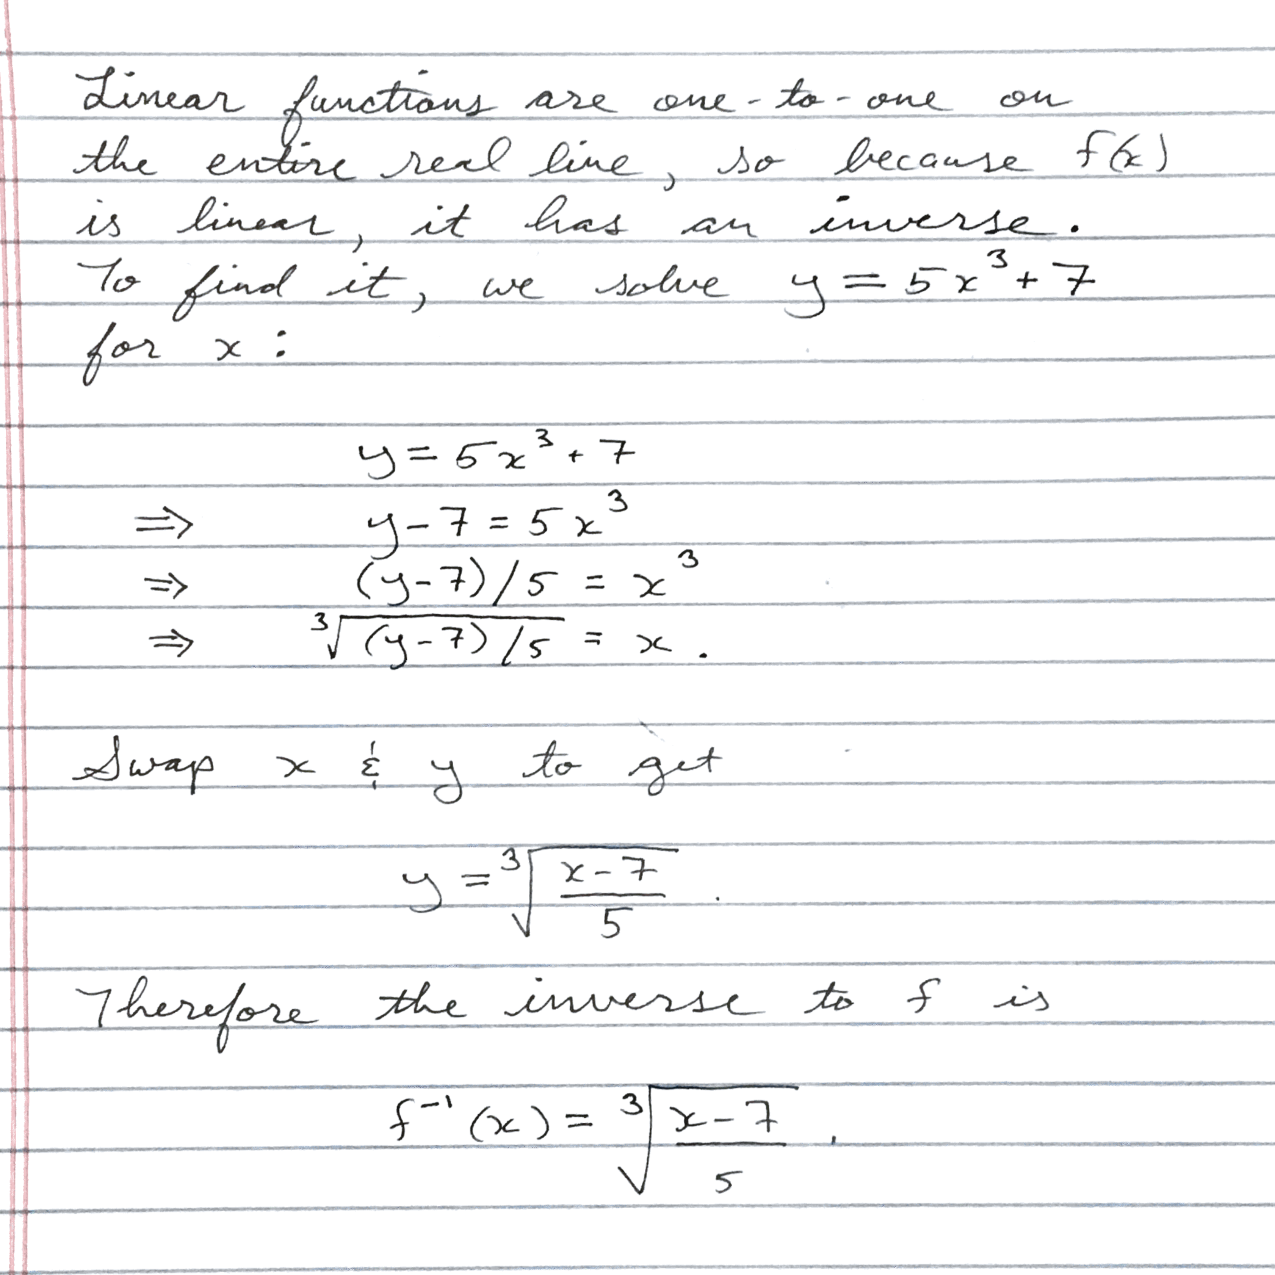
\includegraphics[scale=0.75]{assets/homework_example_good.pdf}
\end{center}

\noindent
This solution is written in full sentences, each step is
explained, and it can be read left-to-right and
top-to-bottom. Notice that some math expressions are given a
line break and centered.  You may use symbols, such as
`$ \Rightarrow $' which means `which implies that'.
\pagebreak

\noindent
\textbf{Here is a poorly-written solution:}
\begin{center}
  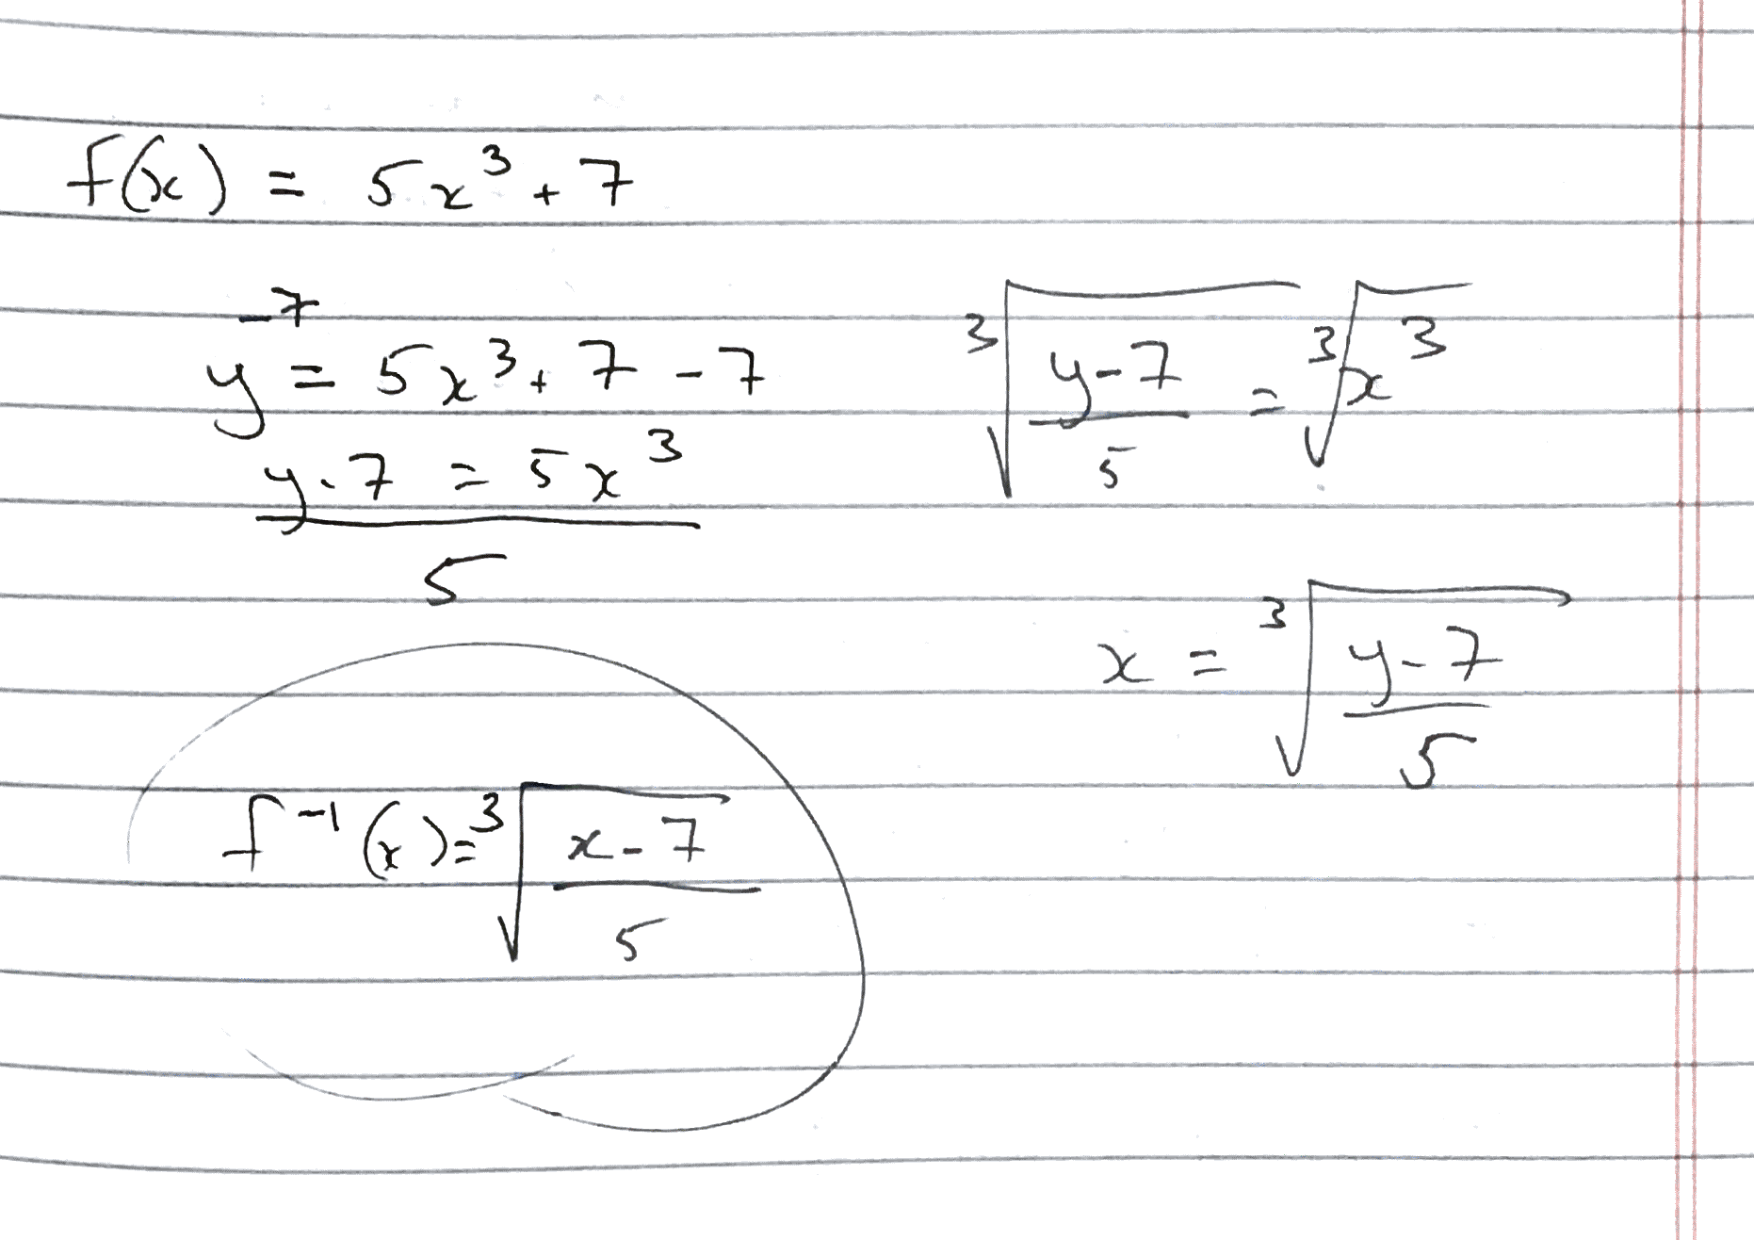
\includegraphics[scale=0.5]{assets/homework_example_bad.pdf}
\end{center}

\noindent
Even though we get the same inverse function as the
well-written, this would receive a 0 grade for the
\emph{written component}.  Nothing is explained and there is
no discernable order to any of the steps. This is scratch
work. It is a perfectly passable first draft and useful for
initially solving the problem. But nobody other than the
person who wrote this would be able to read it.




\end{document}
